%
% This is the LaTeX template file for lecture notes for EE 382C/EE 361C.
%
% To familiarize yourself with this template, the body contains
% some examples of its use.  Look them over.  Then you can
% run LaTeX on this file.  After you have LaTeXed this file then
% you can look over the result either by printing it out with
% dvips or using xdvi.
%
% This template is based on the template for Prof. Sinclair's CS 270.

\documentclass[twoside]{article}
\usepackage{graphics}
\usepackage{algorithm}
\usepackage{algpseudocode}
\usepackage{qtree}
\usepackage{pgfplots}
\usepackage{tikz-qtree}


\setlength{\oddsidemargin}{0.25 in}
\setlength{\evensidemargin}{-0.25 in}
\setlength{\topmargin}{-0.6 in}
\setlength{\textwidth}{6.5 in}
\setlength{\textheight}{8.5 in}
\setlength{\headsep}{0.75 in}
\setlength{\parindent}{0 in}
\setlength{\parskip}{0.1 in}



%
% The following commands set up the lecnum (lecture number)
% counter and make various numbering schemes work relative
% to the lecture number.
%
\newcounter{lecnum}
\renewcommand{\thepage}{\thelecnum-\arabic{page}}
\renewcommand{\thesection}{\thelecnum.\arabic{section}}
\renewcommand{\theequation}{\thelecnum.\arabic{equation}}
\renewcommand{\thefigure}{\thelecnum.\arabic{figure}}
\renewcommand{\thetable}{\thelecnum.\arabic{table}}
\renewcommand{\O}[1]{$\mathcal{O}(#1)$}
\algnewcommand\algorithmicinput{\textbf{INPUT:}}
\algnewcommand\INPUT{\item[\algorithmicinput]}
\algnewcommand\algorithmicoutput{\textbf{OUTPUT:}}
\algnewcommand\OUTPUT{\item[\algorithmicoutput]}

%
% The following macro is used to generate the header.
%
\newcommand{\lecture}[4]{
   \pagestyle{myheadings}
   \thispagestyle{plain}
   \newpage
   \setcounter{lecnum}{#1}
   \setcounter{page}{1}
   \noindent
   \begin{center}
   \framebox{
      \vbox{\vspace{2mm}
    \hbox to 6.28in { {\bf EE 382V: Parallel Algorithms
                        \hfill Summer 2017} }
       \vspace{4mm}
       \hbox to 6.28in { {\Large \hfill Lecture #1: #2  \hfill} }
       \vspace{2mm}
       \hbox to 6.28in { {\it Lecturer: #3 \hfill Scribe: #4} }
      \vspace{2mm}}
   }
   \end{center}
   \markboth{Lecture #1: #2}{Lecture #1: #2}
   %{\bf Disclaimer}: {\it These notes have not been subjected to the
   %usual scrutiny reserved for formal publications.  They may be distributed
   %outside this class only with the permission of the Instructor.}
   \vspace*{4mm}
}

%
% Convention for citations is authors' initials followed by the year.
% For example, to cite a paper by Leighton and Maggs you would type
% \cite{LM89}, and to cite a paper by Strassen you would type \cite{S69}.
% (To avoid bibliography problems, for now we redefine the \cite command.)
% Also commands that create a suitable format for the reference list.
\renewcommand{\cite}[1]{[#1]}
\def\beginrefs{\begin{list}%
        {[\arabic{equation}]}{\usecounter{equation}
         \setlength{\leftmargin}{2.0truecm}\setlength{\labelsep}{0.4truecm}%
         \setlength{\labelwidth}{1.6truecm}}}
\def\endrefs{\end{list}}
\def\bibentry#1{\item[\hbox{[#1]}]}

%Use this command for a figure; it puts a figure in wherever you want it.
%usage: \fig{NUMBER}{SPACE-IN-INCHES}{CAPTION}
\newcommand{\fig}[3]{
			\vspace{#2}
			\begin{center}
			Figure \thelecnum.#1:~#3
			\end{center}
	}
% Use these for theorems, lemmas, proofs, etc.
\newtheorem{theorem}{Theorem}[lecnum]
\newtheorem{lemma}[theorem]{Lemma}
\newtheorem{proposition}[theorem]{Proposition}
\newtheorem{claim}[theorem]{Claim}
\newtheorem{corollary}[theorem]{Corollary}
\newtheorem{definition}[theorem]{Definition}
\newenvironment{proof}{{\bf Proof:}}{\hfill\rule{2mm}{2mm}}

% **** IF YOU WANT TO DEFINE ADDITIONAL MACROS FOR YOURSELF, PUT THEM HERE:

\begin{document}

% declaration of the new block
\algblock{ParFor}{EndParFor}
% customising the new block
\algnewcommand\algorithmicparfor{\textbf{for}}
\algnewcommand\algorithmicpardo{\textbf{do in parallel}}
\algnewcommand\algorithmicendparfor{\textbf{end\ for}}
\algrenewtext{ParFor}[1]{\algorithmicparfor\ #1\ \algorithmicpardo}
\algrenewtext{EndParFor}{\algorithmicendparfor}

%FILL IN THE RIGHT INFO.
%\lecture{**LECTURE-NUMBER**}{**DATE**}{**LECTURER**}{**SCRIBE**}
\lecture{5}{Parallel Prefix}{Vijay Garg}{Van Quach}
%\footnotetext{These notes are partially based on those of Nigel Mansell.}

% **** YOUR NOTES GO HERE:

% Some general latex examples and examples making use of the
% macros follow.  
%**** IN GENERAL, BE BRIEF. LONG SCRIBE NOTES, NO MATTER HOW WELL WRITTEN,
%**** ARE NEVER READ BY ANYBODY.
\section{Parallel Prefix}
Parallel prefix is the scan operation, which takes an associated binary operator, and a set of n elements and returns a . Let exam an example of a parallel prefix. Given an array A:
\[
\begin{array}{c|c|c|c|c}
A & 2 & 11 & 5 & 8\\
\hline
Prefix Sum & 2 & 13 & 18 & 26
\end{array}•
\]

\begin{algorithm}
\caption{Prefix sum - sequential version}
\begin{algorithmic}[1]
\INPUT $A_k, \forall k = 0\ldots n-1$
\OUTPUT{$C_k = \sum_{i=0}^{k} A_i, \forall k = 0\ldots n-1$}
\Procedure {prefix{\_}sum}{\null}
\For{$i \gets 0, n-1$}
	\State $C[i] = A[i]$
\EndFor
\For{$i \gets 0, n-1$}
	\State $C[i] = C[i-1] + A[i]$
\EndFor
\EndProcedure
\end{algorithmic}
\end{algorithm}
We can illutrate sequential version of the algorithm by a tree as below:

\begin{figure}[ht]
\centering

\begin{tikzpicture}
\tikzset{every tree node/.style={align=center,anchor=north}}
\Tree 
[.{$C[2] \bigoplus$}
  [.{$C[1] \bigoplus]$}
	[.{$C[0]$}
	]
	[.{$A[1]$}
	]
  ] 
  [.{$A[2]$}
  ]
]
\end{tikzpicture}

\caption{Tree graph for sequential version of prefix sum}
\end{figure}
\begin{table}[ht]
\[
\begin{array}{c|c|c}
 & T(n) & W(n)\\
\hline
Sequential & $\O{n}$ & $\O{n}$\\
\end{array}
\]
\caption{Time and Work for sequential version}
\end{table}

We can improve the sequential version of prefix by a parallel recursive version (see professor's note). Parallel version of prefix sum:
\begin{algorithm}
\caption{Prefix sum - parallel version}
\begin{algorithmic}[1]
\Procedure {prefix{\_}sum}{\null}
	\ParFor{$i \gets 0, n - 1$}
		\State $C[i] = A[i]$
	\EndParFor
	
	\For{$d \gets 1, n - 1 $ by $d \times 2$}
		\ParFor{$i \gets 1, n - 1$}
			\If{$i - d > 0$}
				\State $C[i] = C[i] + C[i - d]$
			\EndIf
		\EndParFor
	\EndFor
\EndProcedure
\end{algorithmic}
\end{algorithm}
\begin{figure}[H]
\centering

\[
\begin{array}{c|cccc}
Index & 0 & 1 & 2 & 3\\
\hline
A & 2 & 11 & 5 & 8\\
C &  2 & 11 & 5 & 8\\
C, d = 1 & 2 & 13 & 16 & 13\\
C, d = 2 & 2 & 13 & 18 & 26\\
\end{array}
\]
\caption{C's values for each step}
\end{figure}

\begin{table}[ht]
\[
\begin{array}{c|c|c}
 & T(n) & W(n)\\
\hline
Sequential & $\O{\log(n)}$ & $\O{n \times \log(n)}$\\
\end{array}
\]
\caption{Time and Work for parallel version}
\end{table}

We can improve the parallel version to obtain work optimal algorthim by cascading technique. In cascading techinque, we can break input array into $\frac{n}{\log(n)}$ segments of size \O{\log(n)}. We save this implementation for homework



\end{document}





